\thispagestyle{emptyhead}

\section{Installing and setting up R and RStudio}

Before you can start to learn statistics using this workbook, it is required that you have installed both \texttt{R} and RStudio on your computer. \texttt{R} itself is a bare-bones programming environment, and can therefore be hard to learn and navigate without any guidance or visual indications. RStudio is a shell around the \texttt{R} language which offers some guidance and visualizes most of the functionality that \texttt{R} generally hides for users.\\

\texttt{R} is open-source and can be downloaded free-of-charge from \url{https://cran.r-project.org}. While working through this workbook, you will not actually open this program at any time, but you are required to have it installed since it is the engine that RStudio runs on. \\

RStudio is a user-friendly coding environment that makes your life while working with \texttt{R} a little bit easier. RStudio can be freely downloaded from \url{https://rstudio.com}. This is the program that you will be using to write and run your own \texttt{R} code. \\

\vspace*{1cm}

\begin{minipage}{0.4\textwidth}
\textit{1. If you open RStudio for the first
time you will encounter the
following screen:}
\end{minipage}%
\hfill%
\begin{minipage}{0.55\textwidth}
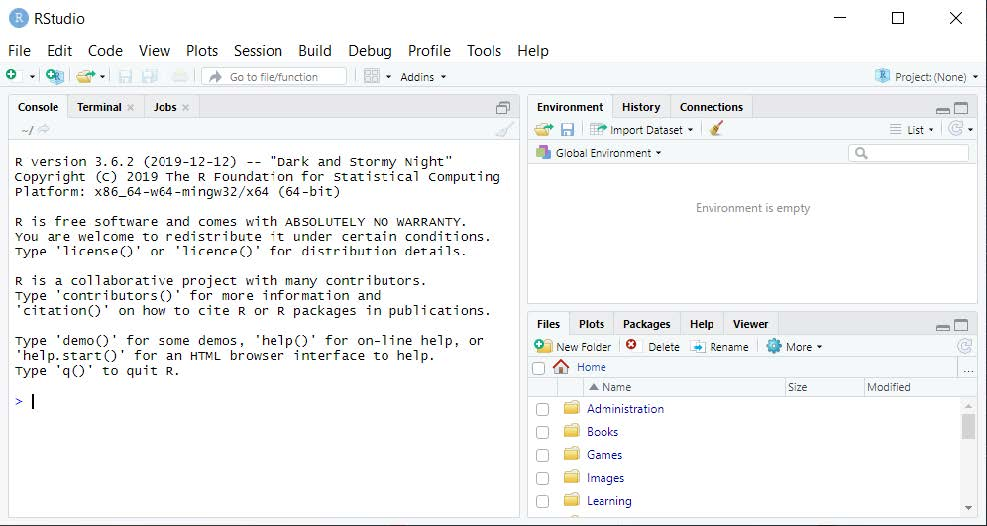
\includegraphics[width=\linewidth]{Files/Images/setup1.jpg}
\end{minipage} \\
\\
\bigskip

\begin{minipage}{0.5\textwidth}
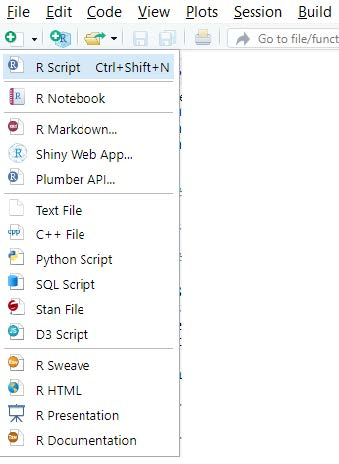
\includegraphics[width=.4\linewidth]{Files/Images/setup2.jpg}
\end{minipage}%
\hfill%
\begin{minipage}{0.4\textwidth}
\textit{2. Press the “New” menu button and choose
“R Script”, or press Ctrl ( $\cmd$ ) + Shift + N to
open a new \texttt{R} script.}
\end{minipage} \\
\\
\bigskip

\begin{minipage}{0.4\textwidth}
\textit{3. You can now write and run your
own code in the newly opened
\texttt{R} script. Highlight all code you
want to execute and press
Ctrl ( $\cmd$ ) + Enter or "Run" to run.}
\end{minipage}%
\hfill%
\begin{minipage}{0.55\textwidth}
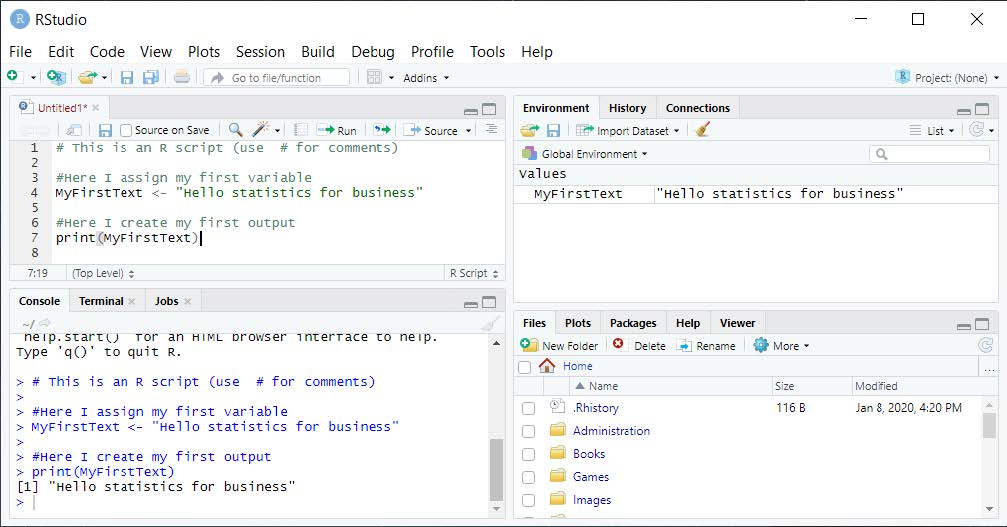
\includegraphics[width=\linewidth]{Files/Images/setup3.jpg}
\end{minipage} \\
\\
\bigskip

\clearpage % Page break
